\chapter{Methodology}
\label{chap:methodology}

As this project is the continuation of work started in the previous semester,
some of the experiments in this project target the same problems as before,
with different methods in an attempt to get better results.
Other experiments target problems not previously attempted with CA-NEAT.

\section{CA-NEAT Implementation}
\label{sec:implementation}
TODO

\begin{figure}
\centering
\begin{multicols}{3}
\begin{enumerate}
    \item Sigmoid
    \item Hyperbolic tangent
    \item Sinusoid
    \item Gaussian
    \item Rectified linear unit
    \item Identity
    \item Clamped
    \item Inverse
    \item Logarithmic
    \item Exponential
    \item Absolute value
    \item Hat
    \item Square
    \item Cube
\end{enumerate}
\end{multicols}
\caption{Possible activation functions}
\label{fig:activations}
\end{figure}

\begin{figure}
\centering
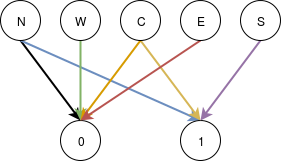
\includegraphics[width=.5\columnwidth]{fig/single_layer_cppn}
\caption
[Example first-generation CPPN with 7 out of 10 possible connections.]
{Example first-generation CPPN with 7 out of 10 possible connections. $N=5$ input nodes corresponds to the "Von Neumann" neighbourhood shape, and $K=2$ output nodes correspond to a binary CA.}
\label{fig:single_layer_cppn}
\end{figure}

The nodes of the evolved CPPNs can have any of the activation functions listed in Figure \ref{fig:activations}.

\section{Novelty Search}
In order to extend CA-NEAT for novelty search, some phenotype value needs to be measured and compared in order to calculate novelty.
The enumerated "string" representation of the transition function was selected for this.
The \textit{Hamming distance} between different strings can then be calculated and used as a measure of novelty distance.

\section{Investigation of Genome Properties}
In order to gain a better understanding of the somewhat opaque GA process,
an experiment was designed with the goal of investigating the development of various properties of the population over time.

The "tricolor morphogenesis" was used as the basis for this experiment, since previous experiments with this problem showed it to be solvable, but not trivially simple for CA-NEAT.
The CA for this problem has $K=4$ cell states and the neighbourhood shape "Von Neumann" ($N=5$) was used.
An initial population of size $P=1000$ was created, with $N$ input nodes, $K$ output nodes and no initial hidden nodes.
This same population was then used as the initial population for five independent runs of $G=100$ generations, with different mechanisms of NEAT in use.
Table \ref{tbl:NEAT_incremental} shows which mechanisms are in use in which runs.

\begin{table}[h]
    \centering
    \caption{TODO}
    \begin{tabular}{c|ccccc}
    Run & Mutation & Crossover & Selection pressure & Speciation & Elitism \\ \hline
    A   & \checkmark        & ~         & ~                  & ~          & ~       \\
    B   & \checkmark        & \checkmark         & ~                  & ~          & ~       \\
    C   & \checkmark        & \checkmark         & \checkmark                  & ~          & ~       \\
    D   & \checkmark        & \checkmark         & \checkmark                  & \checkmark          & ~       \\
    E   & \checkmark        & \checkmark         & \checkmark                  & \checkmark          & \checkmark       \\
    \end{tabular}
    \label{tbl:NEAT_incremental}
\end{table}

Run A is a bit different, since it is not truly a GA run.
Instead the individuals that make up the population are mutated repeatedly, but crossover and elimination is not used.
Run B uses NEAT, however the selection is completely random, so there is no selection pressure.
Run C has selction pressure appropriate for the morphogenesis problem, but does not use the speciation mechanism of NEAT.
Run D is like C, but also uses the speciation mechanism.
And finally, run E uses all mechanisms of NEAT, including a pre-species elitism degree of $E=1$.

100 gens
    - only mutation
    - mutation + crossover, but fitness is constant
        -elitism=0
    - majority problem (do not stop scenario when f==1.0)
        -elitism=0?

investigate
    - lambda spread, mean, mode
    - genome size
    - change in enum-string
        - in terms of mean, median distance and bool(did change?)
    - amount of 'vestigial' nodes

\begin{figure}
\centering
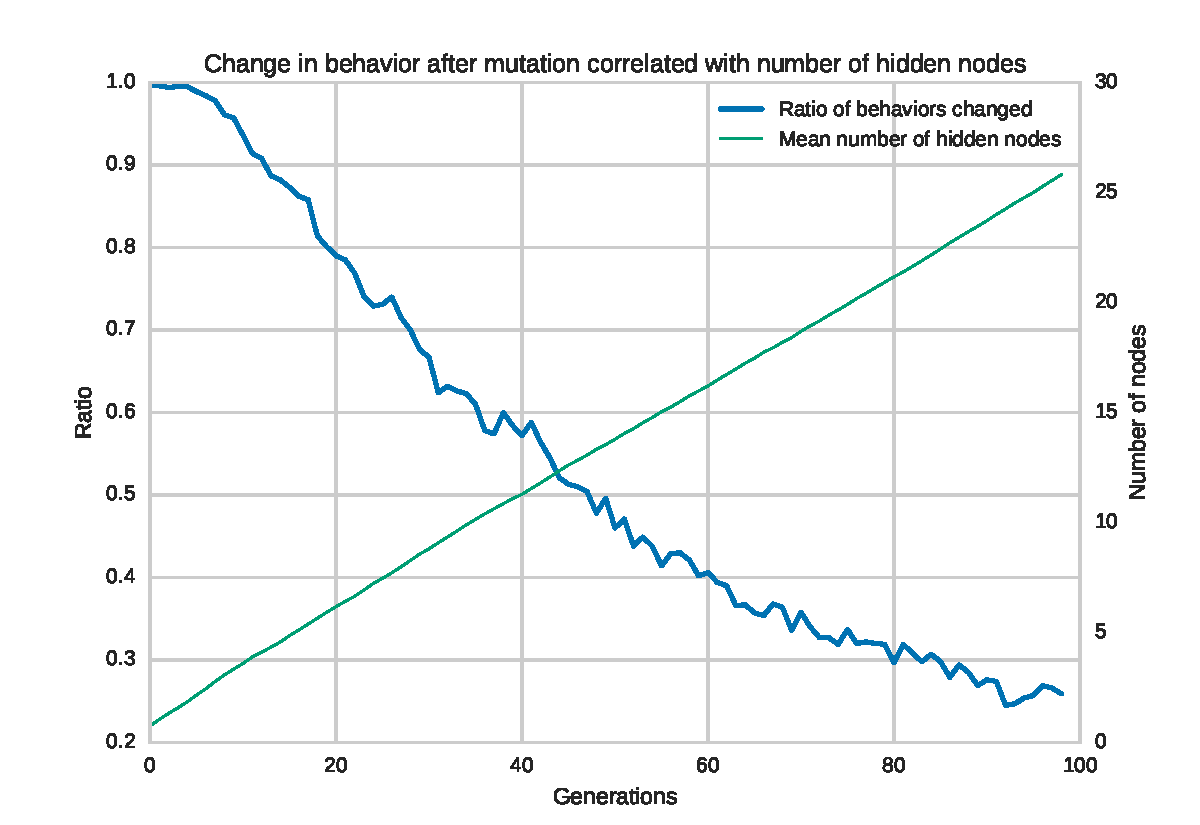
\includegraphics[width=\columnwidth]{fig/mutation_behavior_change}
\caption{TODO}
\end{figure}

\begin{figure}
\centering
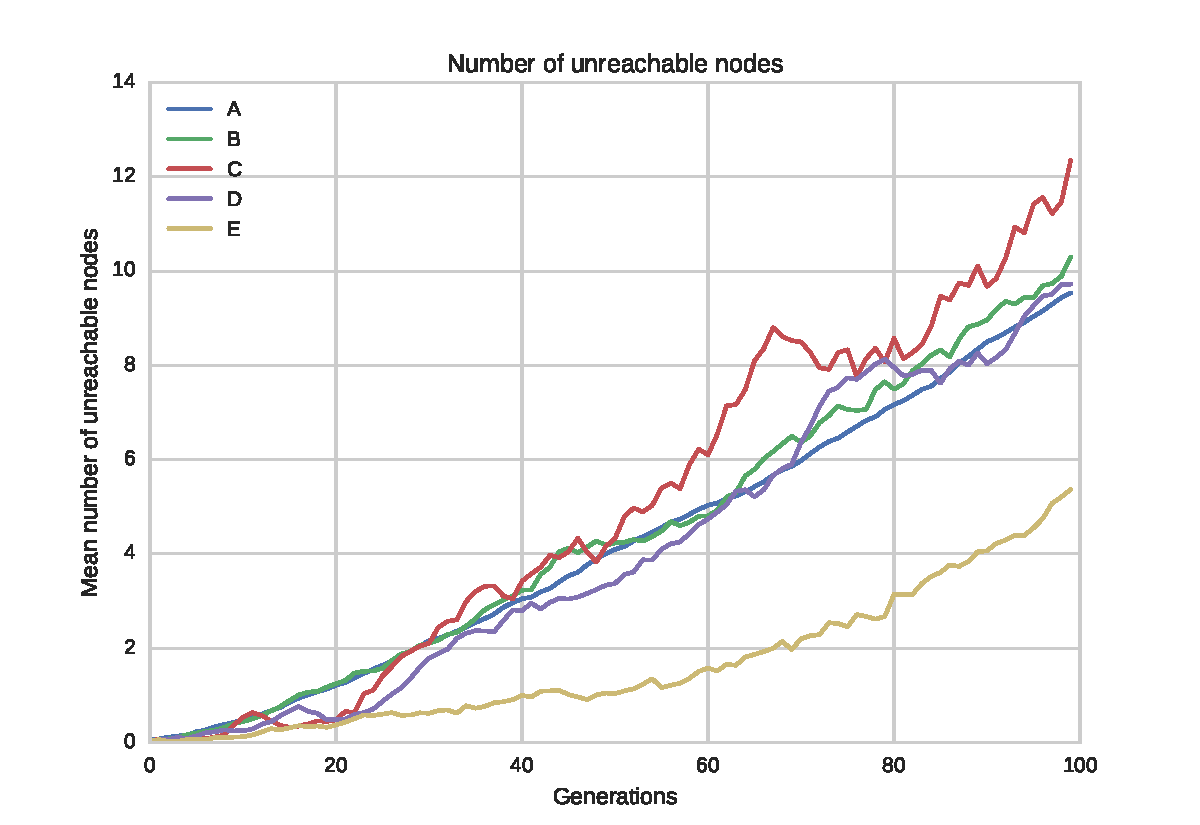
\includegraphics[width=\columnwidth]{fig/vestigial_nodes}
\caption{TODO}
\end{figure}

\begin{figure}
\centering
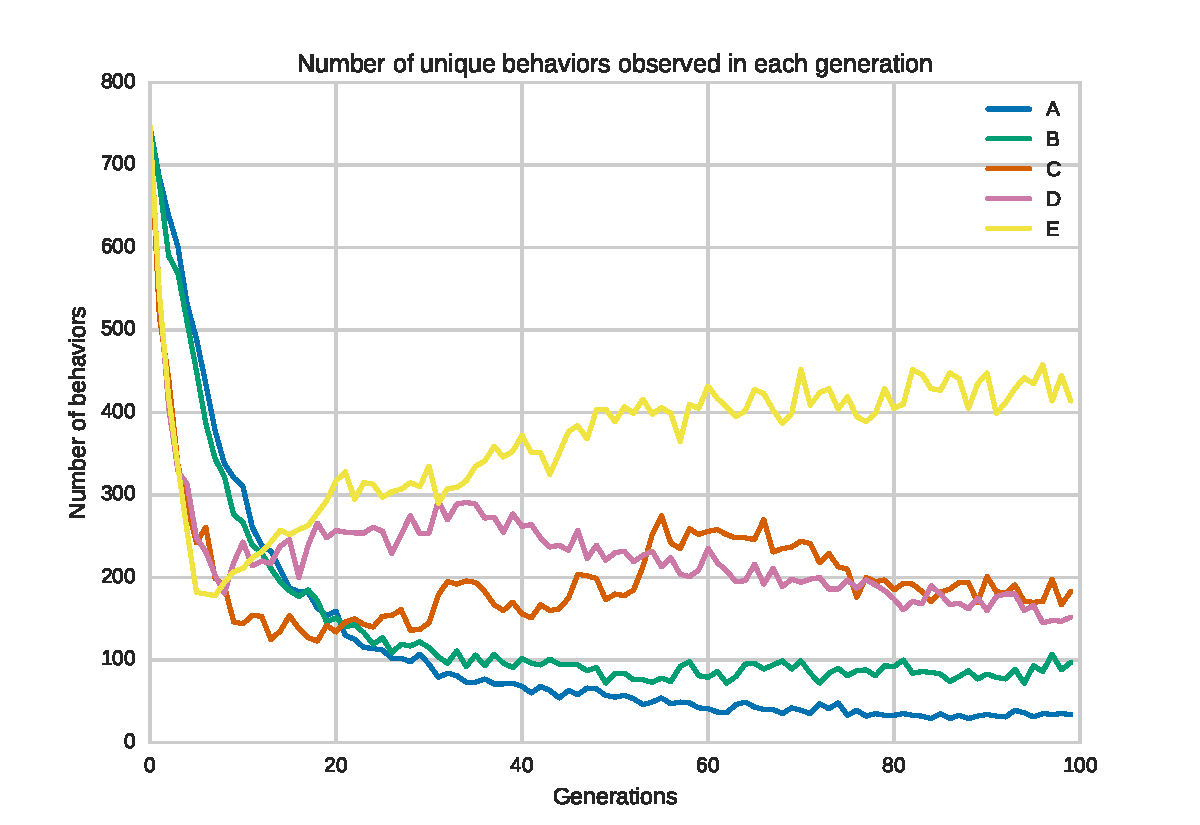
\includegraphics[width=\columnwidth]{fig/unique_behaviors}
\caption{TODO}
\end{figure}

\section{2D Morphogenesis With Coordinate Inputs}
TODO

\section{Majority Problem}
TODO

\section{Synchronization Problem}
Another problem for binary CA is called the \textit{synchronization problem}.
From some arbitrary initial configuration,
the CA should find its way to a two-step cyclic attractor where all cells share the same state in one timestep,
then all share the other state in the next timestep.
It is thus simillar to the majority problem in the way information must be transmitted across the CA in order to coordinate the cells,
but instead of having to "count" cells and landing in a specific point attractor, it finds a cyclic attractor without concern for which of the two states it visits first.

The fitness evaluation function for this experiment is based on the one described in \cite{das1995evolving}, but with some modifications.
$K=100$ random initial CA configurations are generated from a TODO distribution.
Each candidate solution is first tested on $I=25$ initial configurations.
If none of the $I$ configurations results in the desired behavior, a fitness of $0.0$ is reported.
If any of the configurations does result in the desired behavior, the candidate is tested on all $K$ configurations.
The fitness reported is then the ratio of configurations that show the correct behavior.


\section{Firing Squad Synchronization Problem}
TODO

\section{Novelty Search}
In order to extend CA-NEAT for novelty search, some phenotype value needs to be measured and compared in order to calculate novelty.
The enumerated "string" representation of the transition function was selected for this.
The \textit{Hamming distance} between different strings can then be calculated and used as a measure of novelty distance.

